\section{Ejercicio 1}

\subsection{Descripci\'on del problema}

En un puesto de control, se posee informaci\'on sobre los d\'ias de llegada de un n\'umero $n$ de camiones. Cada cami\'on pasa una vez, y es posible que en un d\'ia determinado puedan pasar varios de ellos. Sabiendo esto, se quiere contratar a un inspector que los revise. Este inspector s\'olo puede ser contratado por una cantidad fija de $D$ d\'ias consecutivos, por lo cual, para sacar mejor provecho del presupuesto, se desea contratar al inspector en un per\'iodo en el cual pase la mayor cantidad de camiones. Se pide disenar e implementar un algoritmo que resuelva este problema en tiempo estrictamente menor a $O(n^2)$.

\vspace{2mm}

Consideremos el siguiente caso como ejemplo \{$n$ $=$ 5; d\'ias $=$ 8, 6, 4, 11, 1; $D$ $=$ 5\}

\vspace{3mm}

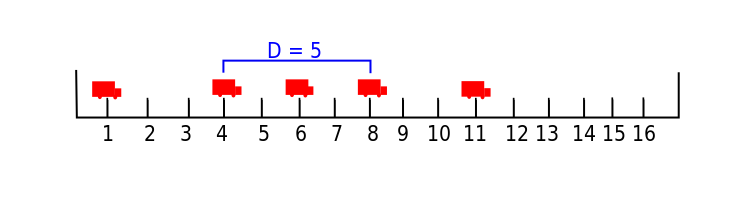
\includegraphics[scale=0.6]{images/intervalo}

\vspace{3mm}

En este caso el per\'iodo del inspector que maximiza la cantidad de camiones es el [4,8] ya que en ning\'un otro intervalo llegan m\'as de 3 camiones, por lo que esa deber\'ia ser el resultado de nuestro algoritmo.

\subsection{Funcionamiento del algoritmo}

\hspace{2mm}

En esta secci\'on daremos una idea informal acerca del funcionamiento de nuestro algoritmo para luego dar paso a las demostraciones formales.

\vspace{2mm}

\subsubsection{Preliminares}

\vspace{2mm}

La entrada del algoritmo es de la forma $D$ $n$ $d1$ $d2$ . . .$dn$, donde $D$ son los d\'ias de contrataci\'on del experto, $n$ la cantidad de camiones, y $d1$, $d2$... $dn$ los d\'ias en los que pasa cada cami\'on, no necesariamente en orden cronol\'ogico.

\vspace{2mm}

Paso 1: El algoritmo ordena los d\'ias en los que vienen los camiones de manera de tener un vector calendario. Este vector de enteros va a representar una sucesi\'on de d\'ias en los que viene al menos un cami\'on. En caso de venir m\'as de un cami\'on el mismo d\'ia, ese d\'ia aparecer\'a tantas veces como camiones vengan.

\vspace{2mm}

\vspace{2mm}

Paso 2: Una vez hecho esto, el algoritmo transforma este vector de d\'ias en un vector de tuplas$<$d\'ia, $\sharp$camiones$>$, donde $\sharp$camiones es la suma acumulada de camiones que llegaron desde el d\'ia 1 hasta ese d\'ia inclusive. De esta forma, se agrupan los d\'ias repetidos, posibilitando las b\'usquedas binarias en el vector, y al tener las sumas acumuladas hasta cada d\'ia, se puede obtener en tiempo constante la cantidad de camiones que llegaron en un intervalo [$a$..$b$], restando la suma acumulada del d\'ia anterior a $a$ a la del d\'ia $b$.

\vspace{2mm}

\subsubsection{Ciclo Principal}

\vspace{2mm}

Antes de seguir, consideremos otro caso posible del problema, en el que hay varios posibles intervalos \'optimos que maximicen la cantidad de camiones.
\{$n$ $=$ 5, d\'ias = 5,1,8,7,6; $D$ $=$ 5\}

\vspace{2mm}

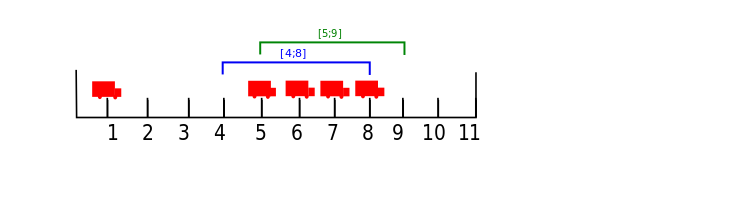
\includegraphics[scale=0.75]{images/intervalo2}

\vspace{2mm}

Vemos que en este caso hay dos intervalos que maximizan la cantidad de camiones (4): [4,8]; [5,9], llam\'mosles $a$ y $b$.

\vspace{2mm}

Seg\'un el enunciado en caso de haber varias soluciones \'optimas debemos devolver cualquiera de ellas. El funcionamiento de nuestro algoritmo hace que devuelva una particular.
Podemos ver que en el intervalo $a$, el primer cami\'on llega el d\'ia 5. Con lo cual el experto es contratado el d\'ia 4 innecesariamente, ya que no llega ning\'un cami\'on ese d\'ia. Si contrat\'aramos al experto el d\'ia 5, podr\'ia revisar todos los mismos camiones que revisaba el intervalo $a$ y tendr\'ia un d\'ia m\'as (el d\'ia 9) para revisar camiones (aunque en este caso no venga ninguno m\'as).

\vspace{2mm}

Siguiendo la l\'inea de pensamiento, cualquier intervalo \'optimo que maximice la cantidad de camiones, puede ser desplazado hacia la derecha de modo que el primer d\'ia en que es contratado el experto sea el primer d\'ia en el que viene un cami\'on en el intervalo original. Todos los camiones que abarcaba el intervalo original van a ser abarcados por el intervalo desplazado, y todos los d\'ias del principio que no eran aprovechados pasan a ser parte del final del intervalo, dando la posibilidad de poder revisar m\'as camiones. 
Por lo cual nuestro algoritmo ni siquiera considerar\'ia la evaluaci\'on del intervalo $a$ y devolver\'ia como resultado el intervalo $b$.


\vspace{2mm}

Esto es clave para entender el funcionamiento y por lo tanto la correctitud de nuestro algoritmo, ya que \'este se limita a considerar el subconjunto de intervalos de longitud $D$ que comienzan en un d\'ia en el que viene un cami\'on. El cardinal de este subconjunto, y por lo tanto la cantidad de intervalos que tiene que evaluar es n.


\vspace{2mm}

 Paso 3: La evaluaci\'on de cada intervalo se produce de la siguiente forma: En cada iteraci\'on, se toma una de las tuplas$<$dia, $\sharp camiones>$, llam\'emosle $i$. La primer componente de la tupla ($i_1$)  es el d\'ia en el que comienza el intervalo. A ese d\'ia, se le suma $D$- $1$. Este n\'umero es \'ultimo d\'ia que el experto revisa, llam\'emosle $f$. 
 
 \vspace{2mm}

Paso 4: A continuaci\'on se realiza una b\'usqueda binaria en el vector para poder obtener la suma acumulada de camiones hasta el d\'ia f. En caso de no existir este d\'ia en el vector se toma la tupla cuyo d\'ia es el menor m\'as cercano a f (Ya que no vienen camiones entre este d\'ia y $f$, la suma acumulada de camiones hasta el d\'ia menor m\'as cercano es igual a la de $f$).
\vspace{2mm}

Paso 5: Una vez obtenida la segunda tupla, se realiza la resta de: la suma acumulada hasta $f$ - la suma acumulada hasta el d\'ia $i$ -1. Esto nos da como resultado la cantidad de camiones que llegan en el intervalo [$i_1$ .. $f$], o en otras palabras la cantidad de camiones que revisa el experto si es contratado desde el dia $i_1$ hasta el $f$. Lo cual es lo que tenemos que maximizar.

\vspace{2mm}

Paso 6: Este resultado se guarda en una variable que se va reemplazando a medida que se itera por cada una de las $n$ tuplas, de forma de encontrar el m\'aximo.

\vspace{2mm}

A continuaci\'on se muestra un pseudoc\'odigo de lo anteriormente explicado.

\vspace{20mm}


\begin{algorithmic}[1]
	
	\Statex
	\Procedure{maximizarCamiones}{int diasInspector, int[] tablaDiaCantidad, int $\sharp$camiones}
	\State $Ordenar (tablaDiaCantidad)$
	\Comment{Paso 1}
	\State $AgruparYAcumular (tablaDiaCantidad)$
	\Comment{Paso 2}
	\State $int \:  maximo \gets -1$
	\State $int \: diaAContratar \gets -1$
	\For{$i \gets 0; i < tablaDiaCantidad.size; i++$}
	\Comment{Ciclo Principal}
		\State $tupla<int, \,int> \, inicio \gets tablaDiaCantidad[i]$
		\Comment{Paso 3}
		\State $int \: diaFinal \gets inicio.first + diasInspector -1$
		\State $tupla<int, int> final \gets tDC[BusquedaBinaria(tDC,i, diaFinal, tDC.size())]$
		\Comment{Paso 4}
		\State $int \sharp camionesDelIntervalo \gets final.second - tablaDiaCantidad[i-1].second$
		\Comment{Paso 5}
		\If{$\sharp camionesDelIntervalo > maximo$}
		\Comment{Paso 6}
			\State $maximo \gets camionesDelIntervalo$
			\State $diaAContratar \gets inicio.first$
		\EndIf
	\EndFor
	\State $return <diaAContratar, \, maximo>$
	\EndProcedure
	\Statex
	\end{algorithmic}

Nota: en el paso 4 abreviamos tablaDiaCantidad por tDC para una mejor lectura.

Se puede ver una implementaci\'on del algoritmo en la secci\'on \ref{codigo_1}.

\subsection{Demostraci\'on de correctitud}

Definamos algunos conceptos:

\vspace{2mm}

El algoritmo recibe $n$ naturales, con posibilidad de repetidos, que representan los d\'ias en los que llegan los camiones. Podemos representar formalmente esto con un multiconjunto de naturales, implementado con un vector al que llamaremos $calendario$. Por cada d\'ia, vienen tantos camiones como cantidad de repeticiones tenga en el multiconjunto.

\vspace{2mm}

Podemos definir formalmente las funciones $"cantCamionesDia"$, que dado un vector calendario y un dia devuelve la cantidad de camiones que llega ese d\'ia y $"cantCamionesIntervalo"$ que dado un calendario y dos d\'ias devuelve la cantidad de camiones que llegan entre esos d\'ias.

\begin{align*}
cantCamionesDia(calendario, dia) = cantRepeticiones(calendario, dia) 
\end{align*}

Donde cantRepeticiones es una funci\'on can\'onica de los multiconjuntos que dado un natural y un multiconjunto devuelve su cantidad de apariciones en \'el.

\vspace{2mm}

Definimos intervalo a un par de naturales $<x,y>$ con $x$ $\leq y$.

\begin{align*}
cantCamionesIntervalo(calendario, intervalo) = \sum_{i=intervalo_1}^{intervalo_2}( cantRepeticiones(calendario, i) ) 
\end{align*}

Esto representa la 'cantidad de camiones que llega en un intervalo'. Finalmente definamos la funci\'on principal $maximizarCamiones$, que es la formalizaci\'on matem\'atica del algoritmo. Los par\'ametros de la funci\'on son: el calendario y los d\'as que se contrata el inspector. Llamemos $I_D$ a todos los intervalos posibles entre $1$ y $max(calendario)$ de longitud D. N\'otese que al ser naturales este es un conjunto finito.

\begin{align*}
\begin{split}
maximizarCamiones(calendario, D)  =  i \in I_D / \forall x in I_D, cantCamionesIntervalo(calendario,x)& \leq  \\ cantCamionesIntervalo(i)
\end{split}
\end{align*}

\subsubsection{Correctitud de la acumulaci\'on}

Nuestro algoritmo manipula los d\'ias entrada, primero orden\'andola (la correctitud de esto est\'a asegurada por la documentaci\'on del lenguaje) y luego la transforma en un vector de tuplas, cuyas primeras componentes son los d\'ias anteriormente mencionados y las segundas componentes son la suma acumulada de camiones que llegan desde el d\'ia 1 hasta el d\'ia respectivo de su primera componente. Necesitamos probar que esta acumulaci\'on se realiza de manera correcta.

 \vspace{2mm}

Definamos formalmente la funci\'on $acumDias$ que toma un calendario y un d\'ia $d$ y devuelve la suma acumulada de camiones que llegaron desde el d\'ia 1 hasta $d$.

\begin{align*}
acumDias(calendario, dia) = \sum_{i=1}^{dia}(cantCamionesDia(calendario, i))
\end{align*}


Definido esto, vemos que podemos calcular la cantidad de camiones de un intervalo $<x, y>$ haciendo la resta:
\begin{align*}
acumDias(calendario, y) - acumDias(calendario, x-1)
\end{align*}

Probemos esto. Por definici\'on de $acumDias$:

\begin{align*}
 acumDias(calendario, y) -  acumDias(calendario,  x-1) =  \sum_{i=1}^{y}&(cantCamionesDia(calendario, i) -\\ \sum_{j=1}^{x-1}(cantCamionesDia(calendario, j)
\end{align*}
		Dado que es un intervalo, $ x \leq $ entonces:

\begin{align*}
\sum_{i=1}^{y}(cantCamionesDia(calendario, i) = \sum_{i=1}^{x-1}(cantCamiones&Dia(calendario, i) + \\ \sum_{i=x}^{y}(cantCamionesDia(calendario, i)
\end{align*}


 Si reeemplazamos en la anterior ecuaci\'on, nos queda que:


\begin{align*}
 acumDias(calendario, y) -  acumDias(calendario, x-1) = &\\  \sum_{i=1}^{x-1}(cantCamionesDia(calendario, i) + \\ \sum_{i=x}^{y}(cantCamionesDia(calendario, i)  - \\\sum_{j=1}^{x-1}(cantCamionesDia(calendario, j)
\end{align*}


Cancelando, nos queda:

\vspace{3mm}
\begin{align*}
\sum_{i=x}^{y}(cantCamionesDia(calendario, i) = cantCamionesIntervalo(calendario, <x, y>)
\end{align*}
\vspace{3mm}

Por definici\'on de $cantCamionesIntervalo$.

\vspace{2mm}



Ahora nos queda probar que nuestro algoritmo calcula correctamente la acumulaci\'on durante el ciclo. Veamos el c\'odigo.

\vspace{4mm}


\begin{algorithmic}[1]
	
	\Statex
	\Procedure{agruparYAcumular}{int entrada[]}	
	\State$vector<pair<int, int> > \: tablaDiaCantidad;$
	\State$int \: longuitud = entrada.size();$
	\State$tablaDiaCantidad.reserve(longuitud)$
	\State$int \: i=0;$
	\State$int \: acumulador = 0;$
	\While{$i < longuitud$}
		\State $acumulador++;$
		\If{$(entrada[i] != entrada[i+1]) || (i==longuitud-1)$}
			\State $pair<int, int> par = make\_pair(entrada[i], acumulador);$
			\State $tablaDiaCantidad.push\_back(par);$
		\EndIf
		\State$i++;$
	\EndWhile
	\EndProcedure
	\Statex
	\end{algorithmic}



\vspace{4mm}

El algoritmo reserva el vector de tuplas. Paso seguido declara el indice $i$ para iterar hasta $entrada.size()$ con lo cual vemos que itera sobre todos los d\'ias. Se declara el entero $acumulador$ para guardar la suma acumulada de los d\'ias en el vector.

\vspace{4mm}

Veamos el ciclo. El invariante del ciclo que tenemos es que, en cada iteraci\'on, $acumulador = \sum_{j=1}^{i-1}(cantRepeticiones(entrada[0..i), entrada[j])) $, es decir contiene la cantidad de apariciones en el vector de entrada de todos los d\'as hasta el que estamos iterando, y  $ \forall x \in entrada[0..\phi(entrada[i])] \exists y \in tablaDiaCantidad, y_1 = x \land y_2 = \sum_{j=1}^{x}(cantCamionesDia(entrada, j) \land ordenado(tablaDiaCantidad) $ , es decir, en cada iteracion, por cada d\'ia que est\'e en entrada hasta el anterior d\'ia a $i$ en el que viene un cami\'on (la funcion $\phi$ devuelve el \'indice anterior a la primera aparici\'on de entrada[i]) tablaDiaCantidad va a tener una tupla, con ese d\'ia como primer componente y la acumulaci\'ion de camiones que llegaron como segunda componente, y est\'a ordenado.

\vspace{4mm}

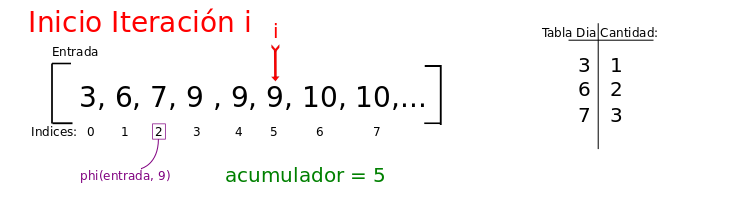
\includegraphics[scale=0.6]{images/iteracioni}

\vspace{4mm}

Suponemos que vale el invariante al comenzar el ciclo. En (7) se le suma 1 a acumulador. Podemos ver que en caso de no valer la guarda del if, no se realizan modificaciones a tablaDiaCantidad, y al final del ciclo (12) se le suma 1 a i. Por lo cual esto valida a acumulador (que suma 1 m\'as al igual que el \'indice), y se reestablece la segunda parte del invariante, al ser $entrada[i] = entrada[i+1]$, la funci\'on $\phi$ va a devolver el mismo n\'umero que en la iteraci\'on anterior, y tablaDiaCantidad no recibi\'o modificaciones.
\vspace{4mm}

En caso de valer la guarda del if, significa que $(entrada[i] != entrada[i+1]) || (i==longuitud-1)$. Si se da la primera condici\'on, acumulador tambi\'en vale al finalizar el ciclo ya que suma 1 junto con el \'indice. La segunda parte del invariante se reestablece, ya que se agrega la nueva tupla $<entrada[i], acumulador>$ a tablaDiaCantidad. La funci\'on $\phi$ en la pr\'oxima iteraci\'on va a devolver el valor de $i$ actual,  valiendo que $ \forall x \in entrada[0..\phi(entrada[i])]$, existe una tupla en tablaDiaCantidad, en particular para $entrada[i]$ es la que acabamos de agregar. La segunda componente de la nueva tupla va a ser igual a $acumulador = \sum_{j=1}^{i-1}(cantRepeticiones(entrada[0..i), entrada[i-1]))$ lo que es igual trivialmente a $ \sum_{j=1}^{x}(cantCamionesDia(entrada, j)$ por definici\'on de $cantCamionesDia$ y porque al estar ordenada $entrada$, no va a haber m\'as apariciones de el d\'ia de la nueva tupla en $entrada[i+1..0]$.

En caso de valer la segunda condici\'on, llegamos al elemento final de entrada por lo cual tenemos que agregarlo a tablaDiaCantidad, y al ser el elemento final ya no va a haber m\'as apariciones de \'el, por lo tanto no va a haber m\'as camiones que lleguen ese d\'ia, lo cual reestablece trivialmente los invariantes.

\vspace{4mm}

Con esto queda demostrado la correctitud del c\'alculo de este vector de tuplas, y sus propiedades.

\vspace{4mm}

\subsubsection{Correctitud de la reducci\'on del dominio}

Es necesario demostrar que la reducci\'on de los intervalos a analizar que realiza el algoritmo es correcta, es decir, que del conjunto de soluciones \'optimas del problema, nuestro algoritmo va a poder devolver efectivamente una de ellas. Nuestro algoritmo solamente eval\'u aquellos intervalos de longitud $D$ que comienzan con un d\'ia en el que viene al menos un cami\'on. Es bastante intuitivo pensar que, cualquier intervalo $<x,y>$ puede ser "mejorado" si se le realiza un "corrimiento a derecha" hasta el primer d\'ia en el que venga un cami\'on en el intervalo. De esta forma no se pierde ningun cami\'on y se abre la posibilidad de que vengan m\'as despues, ya que se aprovecha mejor la longitud del intervalo. 

\vspace{2mm}


Dicho formalmente, sea $c$ un natural tal que $ x \leq c \leq y$ y $cantCamionesDia(calendario, c) \geq 1$ y $\forall i \in [x..y], cantCamionesDia(calendario, i) \geq 1 \Rightarrow c \leq i $, entonces podemos transformar al intervalo $<x,y>$ en el intervalo $<c,c+D>$ y asegurarnos que $cantCamionesIntervalo(calendario, <x,y>) \leq  cantCamionesIntervalo(calendario, <c,c+D>)$.

\vspace{2mm}

Para demostrar que nuestro algoritmo realiza correctamente la reducci\'on del dominio, basta probar que del conjunto de intervalos de longitud D $\subset$ $I_D$ que son soluciones \'optimas, esta reducci\'on deja al menos uno (ya que se pide devolver s\'olo uno).

\vspace{2mm}

Necesitamos probar que para cualquier soluci\'on \'optima, podemos "construirnos" otra soluci\'on \'optima desplaz\'andola a la derecha tal que la cantidad de camiones que lleguen en los dos intervalos sea la misma, y dado que el nuevo intervalo comienza en un d\'ia en el que viene el cami\'on, va a ser evaluada por nuestro algoritmo.

Sea $\alpha = <x, y>$ una soluci\'on \'optima, es decir,
\begin{align*}
 cantCamionesIntervalo(calendario, \alpha) = maximizarCamiones(calendario, D) \land y - x = D
 \end{align*}
 Sea $c$ el natural antes descripto. Sea $\beta = <c, c+D>$. Como $\forall i \in [x..y], cantCamionesDia(calendario, i) \geq 1 \Rightarrow c \leq i $ entonces $i \in [c..c+D]$, ya que por transitividad  $x \leq c \leq i \leq y \leq c + D$. Esto se traduce a que todo d\'ia i del intervalo $\alpha$ en el que viene un cami\'on est\'a pertenece al el intervalo $\beta$. 

 \vspace{2mm}

 Como demostramos que dada una soluci\'on \'optima cualquiera podemos construirnos otra tal que pase la misma cantidad de camiones y comience en un d\'ia en el que viene uno, falta demostrar que nuestro algoritmo efectivamente eval\'ua todos los intervalos posibles que comienzan en un d\'ia en el que viene un cami\'on. Podemos verificar esto trivialmente viendo esta porci\'on del ciclo principal c\'odigo fuente.

 
\begin{algorithmic}[1]
	
	\Statex
		
	\State$for (int i = 0; i < tablaDiaCantidad.size(); ++i)$

		\State $ \: \: \: \: \: \: \: \: \:pair <int, \,int> \, target = tablaDiaCantidad[i]$
		
	


	\Statex
	\end{algorithmic}



	

  \vspace{2mm}

  Vemos que el ciclo itera de 0 a la longitud del vector de tuplas, es decir, eval\'ua todos los intervalos por los que pasa un cami\'on. 


\vspace{4mm}

\subsubsection{Correctitud del c\'alculo de los camiones de un intervalo}

Vamos a demostrar ahora que efectivamente el c\'alculo de la cantidad de camiones en un intervalo dado es correcta. Para calcularla, nuestro algoritmo realiza la resta antes propuesta: $acumDias(calendario, intervalo_1) - acumDias(calendario, intervalo_2 -1) = $

\vspace{4mm}

 Veamos la secci\'ion del ciclo principal del c\'odigo que se encarga de realizar esta tarea. Realizaremos la demostraci\'on sobre el pseudoc\'odigo para abstraernos de los iteradores y dem\'as inconveniencias del c\'odigo fuente, pero es f\'acil comprobar que ambos c\'odigos son equivalentes. 
 \vspace{2mm}


\begin{algorithmic}[1]
	
	\State $tupla<int, \,int> \, inicio \gets dias[i]$
	\State $int \: diaFinal \gets inicio.first + diasInspector -1$
	\State $tupla<int, \, int> final \gets dias[BusquedaBinaria(dias,i, diaFinal, dias.size())]$
	\State $int \sharp camionesDelIntervalo \gets final.second - dias[i-1]$
	
	\end{algorithmic}

	 \vspace{2mm}

Tomamos una tupla del vector, llamada $inicio$ (1). En su primer componente $inicio_1$ tenemos el inicio del intervalo que queremos evaluar. Para tomar el intervalo de longitud $D$ (diasInspector) que comienza en $inicio_1$, calculamos el final del intervalo como $ diaFinal = inicio_1 + D - 1$ (2). Ya tenemos el intervalo a evaluar. Entonces, para ser correcto, nuestro algoritmo deber\'ia calcular $acumDias(entrada,  diaFinal) - acumDias(entrada, inicio_1 -1)$.

\vspace{2mm}

En (3), el algoritmo realiza una b\'usqueda binaria sobre $dias$, buscando la tupla cuya primer componente sea $diaFinal$. De esta forma, en su segunda componente tenemos la suma acumulada de camiones hasta el dia final del intervalo y podriamos realizar la resta propuesta. La funci\'ion $BusquedaBinaria$ (upperBound) nos garantiza el \'indice del primer elemento mayor a $diaFinal$, al restarle uno, obtenemos o bien el \'indice de la tupla cuyo primer componente es $diaFinal$, o el \'indice de la tupla cuyo primer componente es el mayor n\'umero menor a $diaFinal$ en caso de \'este no existir. Llamamos a esta tupla $final$.

Finalmente (4), realizamos la resta $final_2 - dias[i-1]_2$. Gracias a la demostraci\'on anterior, esto podr\'ia traducirse como $ \sum_{k=1}^{final_1}(cantCamionesDia(entrada, k) - \sum_{j=1}^{dias[i-1]_1}(cantCamionesDia(entrada, j)$. Esto es igual a $acumDias(entrada, diaFinal) - acumDias(entrada, inicio_1)$, por los siguientes argumentos:

\vspace{4mm}

Veamos ahora que  $acumDias(entrada, diaFinal) = \sum_{k=1}^{final_1}(cantCamionesDia(entrada, k)$
\vspace{4mm}

Por definici\'on $acumDias(entrada, diaFinal) = \sum_{j=1}^{diaFinal}(cantCamionesDia(entrada, j)$. Si $diaFinal$ se encontraba en el calendario, entonces la b\'usqueda binaria nos devolvi\'o el \'indice de la tupla cuya primer componente es $diaFinal$, entonces $final_1 = diaFinal$, y vale la igualdad. En caso de no existir $diaFinal$ en el calendario, la b\'usqueda nos brinda el \'indice del primer elemento mayor a $diaFinal$, a lo cual rest\'andole 1 obtenemos el  mayor n\'umero menor a $diaFinal$. Esto significa que $\forall x \in [final_1 .. diaFinal], cantCamionesDia(entrada, x) = 0$. Con lo cual podemos extender la sumatoria desde $final_1$ hasta $diaFinal$, haciendo valer la igualdad.

\vspace{2mm}

Veamos que  $acumDias(entrada, inicio_1 -1) = \sum_{k=1}^{dias[i-1]}(cantCamionesDia(entrada, k)$. Por (1), $inicio_1$ = $dias[i]_1$. En caso de existir el d\'ia anterior a $inicio_1$, entonces $inicio_1 - 1 = dias[i - 1]_1$ y vale la igualdad. En caso de no existir, $dias[i-1]_1$ es el mayor n\'umero de los menores a $inicio_1$. Esto significa que $\forall x \in [dias[i-1]_1.. inicio_1-1], cantCamionesDia(entrada, x) = 0$ con lo cual puedo extender la sumatoria hasta $inicio_1-1$ y hacer avaler la igualdad.

\vspace{2mm}

Con esto demostramos que el algoritmo calcula correctamente la funci\'on que calcula la cantidad de camiones de un intervalo.



\subsubsection{Correctitud del c\'alculo del m\'aximo}

Nos queda demostrar que es correcto el c\'alculo del m\'aximo. Veamos la secci\'on del c\'odigo que calcula esto. 
\begin{algorithmic}[1]
\Statex
	\State $int \: maximo=-1;$
	\State $int \: diaAContratar=-1;$
	\For{uint i = 0; i < dias.size(); ++i}
	    \State $pair<int, int> inicio = dias[i];$

	    \State$... procesamiento \: y \: busqueda.... $
		
		\State $int \: cantCamionesDelIntervalo = (final.second-resta;$
		\If{$cantCamionesDelIntervalo>maximo$}
			\State $maximo=cantCamionesDelIntervalo;$	
			\State $diaAContratar = dias[i].first;$
		\EndIf
	\EndFor
	\State $return \: par<diaAContratar, maximo>;$
	\Statex

	\end{algorithmic}

	Podemos ver que en cada iteraci\'on, tenemos un condicional tal que si $cantCamionesDelIntervalo>maximo$ se reemplaza el m\'aximo anterior por el nuevo y el d\'a contratar. Se itera hasta el final del arreglo, por lo que la elecci\'on del m\'aximo es correcta.


\subsection{Cota de complejidad}

Lo primero que hace nuestro algoritmo es ordenar el vector de entrada. Seg\'un la documentaci\'on del lenguaje, esto se realiza en $O(n\, log \, n)$. Acto seguido nuestra funci\'on $acumularYAcumular$ reserva un vector de longitud n ($O(n)$) y realiza n iteraciones sobre el vector de entrada, en la que puede verse que realiza todas operaciones de tiempo constante (la documentaci\'on del lenguaje nos asegura esta complejidad para $make\_pair$ y $push\_back$), por lo que el ciclo es de complejidad $O(n)$. Se declaran algunas variables (tiempo constante), y finalmente se realiza el ciclo principal, en el cual se recorre de 0 a dias.size(), realizando todas operaciones de tiempo constante excepto la $BusquedaBinaria$, cuya documentaci\'on (upperBound) nos asegura tiempo logar\'itmico. Esto nos da una complejidad de $O(dias.size() \, log \, dias.size())$. Pero dado que $dias.size() \leq n$, podemos acotar por $n$ lo que nos deja una complejidad para el algoritmo (omitiendo constantes) de $O(n\, log \, n) + O(n)+  O(n) + O(n\, log \, n) = O(n\, log \, n) $.


